\documentclass[12pt, a4paper]{article} %determina o tamanho da fonte, o tipo de papel e o tipo de documento.

\setlength{\parindent}{1.0 cm} %tamanho do espaço para começar o parágrafo.
\setlength{\parskip}{0.5cm} %tamanho do espaço entre os parágrafos.

%Aqui ficam os pacotes utilizados para formatação do documento de modo geral:

\usepackage[utf8]{inputenc} 
\usepackage{indentfirst} %Coloca espaços nos inícios de parágrafos automaticamente. 
\usepackage[brazilian]{babel} %
\usepackage{amsmath}
\usepackage[hmargin=3cm, vmargin=2.5cm, bmargin=2.5cm]{geometry}
\usepackage{multicol}
\usepackage{graphicx} %para poder inserir imagens
\usepackage{subfig}
\usepackage{booktabs} 
\usepackage{hyperref} %para poder adicionar links e hiperlinks
\usepackage{float} %para poder posicionar as imagens


\usepackage{listings} %para poder incluir códigos
\usepackage{xcolor}
\definecolor{codegreen}{rgb}{0,0.6,0}
\definecolor{codegray}{rgb}{0.5,0.5,0.5}
\definecolor{codepurple}{rgb}{0.58,0,0.82}
\definecolor{backcolour}{rgb}{0.95,0.95,0.92}
\lstdefinestyle{mystyle}{
    backgroundcolor=\color{backcolour},   
    commentstyle=\color{codegreen},
    keywordstyle=\color{magenta},
    numberstyle=\tiny\color{codegray},
    stringstyle=\color{codepurple},
    basicstyle=\ttfamily\footnotesize,
    breakatwhitespace=false,         
    breaklines=true,                 
    captionpos=b,                    
    keepspaces=true,                 
    numbers=left,                    
    numbersep=5pt,                  
    showspaces=false,                
    showstringspaces=false,
    showtabs=false,                  
    tabsize=2,
    morecomment={l}[!],
    language=[77]Fortran,
}
\lstset{style=mystyle}

\begin{document} %começa alguma coisa,neste caso, o documento, sempre importante lembrar de colocar o \end{} para não dar erro 
	
	\begin{titlepage}
		\begin{center}
\Huge{Universidade de São Paulo}\\
\large{Instituto de Física de São Carlos}\\
\vspace{20pt}
\vspace{200pt}
\textbf{Lista 3}\\
\vspace{8cm}
		\end{center}

\begin{flushleft}
\begin{tabbing}
Pedro Calligaris Delbem 5255417\\
\end{tabbing}
\vspace{0.5cm}
Professor: Attilio Cucchieri\\		
		\end{flushleft}
	
		\begin{center}
			\vspace{\fill}
	Abril de 2025	
		\end{center}
	\end{titlepage}

%####################################################################### SUMÁRIO
	\tableofcontents 
	\thispagestyle{empty}
	\newpage
%#########################################################################

\section{Runge-Kutta Methods}

    \subsection{Exerc\'icio 1}

        Tarefa: Demonstrar que o erro da interpola\c{c}\~ao linear
        \begin{equation*}
            f(x,y) = \frac{x - x_{n-1}}{h}f_{n} + \frac{x_{n} - x}{h}f_{n-1}
        \end{equation*}
        \'e $\mathcal{O}(h^{2})$

        Demonstra\c{c}\~ao:

        Seja $f(x) \in C^2$ queremos interpolar $f(x)$ entre os pontos $x_{n-1}$ e $x_n = x_{n-1} + h$ utilizando interpolação linear, e estimar o erro:

        \begin{equation*}
            E(x) = f(x) - \tilde{f}(x)
        \end{equation*}

        onde

        \begin{equation*}
            \tilde{f}(x) = \frac{x - x_{n-1}}{h} f(x_n) + \frac{x_n - x}{h} f(x_{n-1})
        \end{equation*}

        Expandimos $f(x_n)$ em série de Taylor ao redor de $x_{n-1}$:

        \begin{equation*}
            f(x_n) = f(x_{n-1} + h) = f(x_{n-1}) + h f'(x_{n-1}) + \frac{h^2}{2} f''(\xi_1), \quad \xi_1 \in (x_{n-1}, x_n)
        \end{equation*}

        Expandimos também $f(x)$ ao redor de $x_{n-1}$:

        \begin{equation*}
            f(x) = f(x_{n-1}) + (x - x_{n-1}) f'(x_{n-1}) + \frac{(x - x_{n-1})^2}{2} f''(\xi_2), \quad \xi_2 \in (x_{n-1}, x)
        \end{equation*}

        Substituímos a expansão de $f(x_n)$ na expressão de $\tilde{f}(x)$:

        \begin{equation*}
            \tilde{f}(x) = \frac{x - x_{n-1}}{h} \left[ f(x_{n-1}) + h f'(x_{n-1}) + \frac{h^2}{2} f''(\xi_1) \right] + \frac{x_n - x}{h} f(x_{n-1})
        \end{equation*}

        Logo

        \begin{equation*}
            \tilde{f}(x) = \frac{x - x_{n-1}}{h} f(x_{n-1}) + (x - x_{n-1}) f'(x_{n-1}) + \frac{(x - x_{n-1}) h}{2} f''(\xi_1) + \frac{x_n - x}{h} f(x_{n-1})
        \end{equation*}

        Como $x_n = x_{n-1} + h$, temos $x_n - x = h - (x - x_{n-1})$ - assim:

        \begin{equation*}
            \tilde{f}(x) = \left( \frac{x - x_{n-1}}{h} + \frac{h - (x - x_{n-1})}{h} \right) f(x_{n-1}) + (x - x_{n-1}) f'(x_{n-1}) + \frac{(x - x_{n-1}) h}{2} f''(\xi_1)
        \end{equation*}

        Segue que:

        \begin{equation*}
            \tilde{f}(x) = f(x_{n-1}) + (x - x_{n-1}) f'(x_{n-1}) + \frac{(x - x_{n-1}) h}{2} f''(\xi_1)
        \end{equation*}

        Fazendo a subtração entre $f(x)$ e $\tilde{f}(x)$, obtemos:

        \begin{align*}
        f(x) - \tilde{f}(x)
        &= \left[ f(x_{n-1}) + (x - x_{n-1}) f'(x_{n-1}) + \frac{(x - x_{n-1})^2}{2} f''(\xi_2) \right] \\
        &\quad - \left[ f(x_{n-1}) + (x - x_{n-1}) f'(x_{n-1}) + \frac{(x - x_{n-1}) h}{2} f''(\xi_1) \right] \\
        \end{align*}

        Deste modo:
        \begin{align*}
        f(x) - \tilde{f}(x)
        &= \frac{1}{2} \left[ (x - x_{n-1})^2 f''(\xi_2) - (x - x_{n-1}) h f''(\xi_1) \right] \\
        &= \frac{(x - x_{n-1})}{2} \left[ (x - x_{n-1}) f''(\xi_2) - h f''(\xi_1) \right]
        \end{align*}

        Podemos reescrever esse erro como:

        \begin{equation*}
        f(x) - \tilde{f}(x) = -\frac{(x - x_{n-1})(x - x_n)}{2} f''(\tilde{\xi})
        \quad \text{para algum } \tilde{\xi} \in (x_{n-1}, x_n)
        \end{equation*}

        onde usamos que $(x - x_{n-1})(x - x_n) = (x - x_{n-1})^2 - h(x - x_{n-1})$, e agrupamos os termos com uma média das derivadas.

        Portanto, o erro da interpolação linear de $f(x) \in C^2$ entre dois pontos é dado por:

        \begin{equation*}
        \boxed{
        f(x) - \tilde{f}(x) = -\frac{(x - x_{n-1})(x - x_n)}{2} f''(\xi)
        \quad \text{para algum } \xi \in (x_{n-1}, x_n)
        }
        \end{equation*}

        Como $|(x - x_{n-1})(x - x_n)| \le \frac{h^2}{4}$, então:

        \begin{equation*}
        |f(x) - \tilde{f}(x)| = \mathcal{O}(h^2)
        \end{equation*}

    \subsection{Exerc\'icio 2}

        Tarefa: Resolva a equa\c{c}\~ao
        \begin{equation*}
            \frac{d^{2}y(x)}{dx^{2}} = -4\pi^{2}y(x)
        \end{equation*}
        com as condi\c{c}\~oes iniciais $y(x=0) = 0$ e $y'(x=0) = 0$ usando o algoritimo de Runge-Kutta.

        C\'odigo Escrito:
        \lstinputlisting[language=Fortran]{../L3-5255417-ex-2.f90}

        O c\'odigo foi compilado com o comando:
        \begin{verbatim}
            gfortran L3-5255417-ex-2.f90 -o L3-5255417-ex-2.exe
        \end{verbatim}

        Resultados:
        \begin{figure}[H]
            \centering
            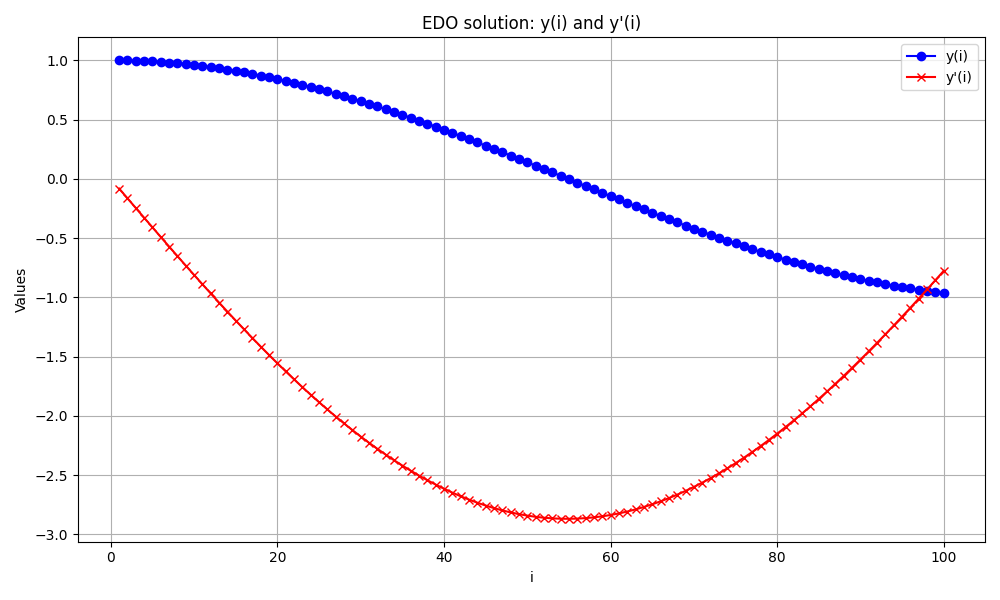
\includegraphics[width=0.8\textwidth]{../images/results-ex-2-2.png}
            \caption{Gr\'aficos de $y(x)$ e $y'(x)$ com h = 0.01}
        \end{figure}
        \begin{figure}[H]
            \centering
            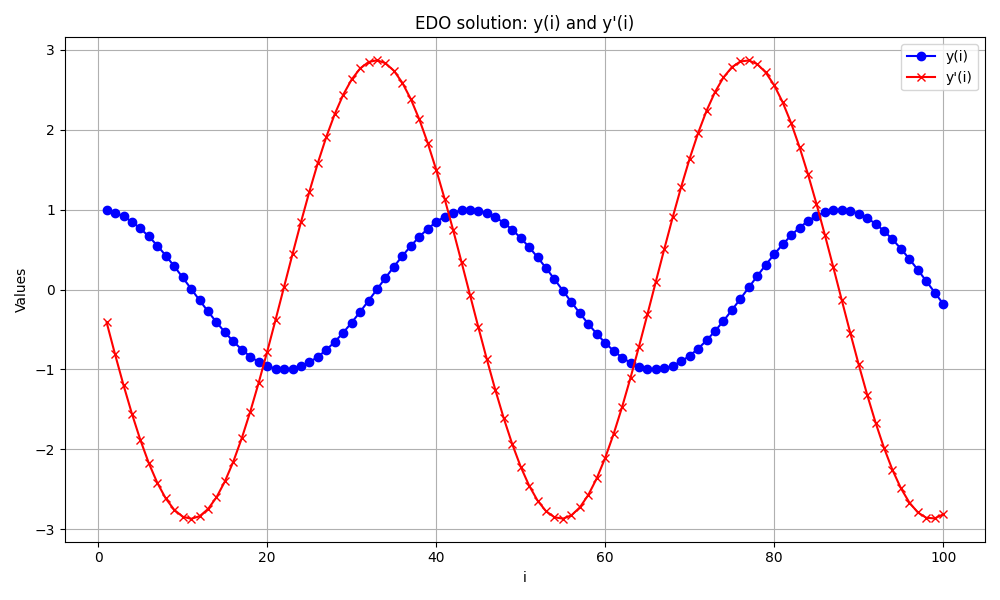
\includegraphics[width=0.8\textwidth]{../images/results-ex-2-4.png}
            \caption{Gr\'aficos de $y(x)$ e $y'(x)$ com h = 0.05}
        \end{figure}
        \begin{figure}[H]
            \centering
            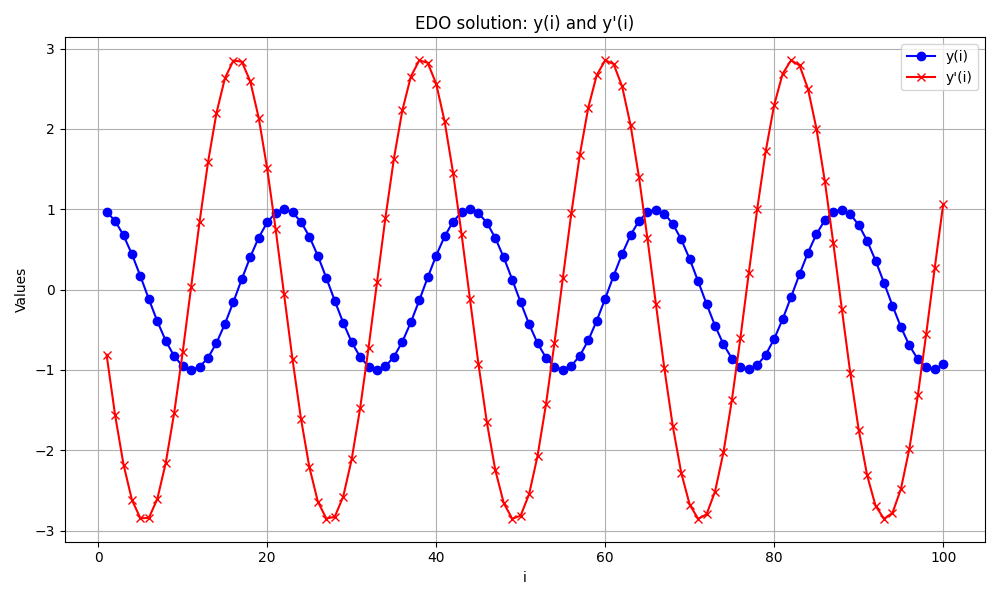
\includegraphics[width=0.8\textwidth]{../images/results-ex-2-1.png}
            \caption{Gr\'aficos de $y(x)$ e $y'(x)$ com h = 0.1}
        \end{figure}
        \begin{figure}[H]
            \centering
            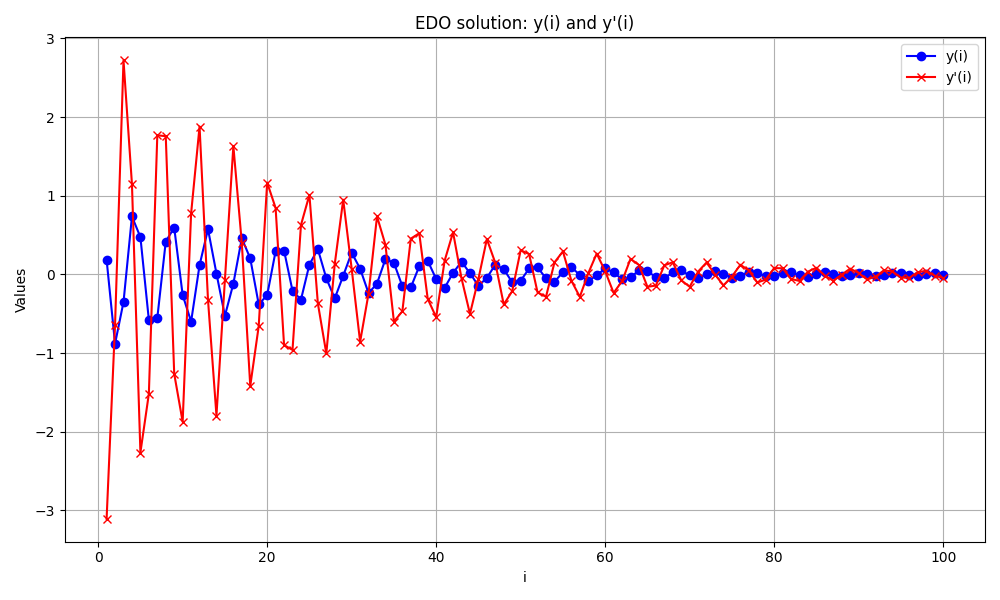
\includegraphics[width=0.8\textwidth]{../images/results-ex-2-3.png}
            \caption{Gr\'aficos de $y(x)$ e $y'(x)$ com h = 0.5}
        \end{figure}

        Nota-se que para os valores de h = 0.1, h = 0.01 e h = 0.05, o resultado obtido s\~ao fun\c{c}\~oes cossenoidais que oscilam de -1 a 1 o que corresponde ao comportamento esperado para a solu\c{c}\~ao da equa\c{c}\~ao diferencial dada. Al\'em disso, as derivadas s\~ao fun\c{c}\~oes senoidais que oscilam de -2$\pi$ a 2$\pi$ o que tamb\'em corresponde ao resultado esperado. Para o valor de h = 0.5, o resultado obtido n\~ao \'e satisfat\'orio, pois a fun\c{c}\~ao n\~ao \'e cossenoidal e a derivada n\~ao \'e senoidal, o que indica que o valor de h = 0.5 \'e muito grande para o algoritmo de Runge-Kutta.

\section{The Numerov Algorithm}

    \subsection{Exerc\'icio 3}

        Tarefa: Resolva a equa\c{c}\~ao
        \begin{equation*}
            \frac{d^{2}y(x)}{dx^{2}} = -4\pi^{2}y(x)
        \end{equation*}
        com as condi\c{c}\~oes iniciais $y(0) = 1$ e $y'(0) = 0$ usando o algoritimo de Numerov. Explique como foram escolhidos os valores iniciais $y_{0}$ e $y_{1}$. Compare o resultado com a solu\c{c}\~ao obtida no exerc\'icio anterior.

        C\'odigo Escrito:
        \lstinputlisting[language=Fortran]{../L3-5255417-ex-3.f90}

        O c\'odigo foi compilado com o comando:
        \begin{verbatim}
            gfortran L3-5255417-ex-3.f90 -o L3-5255417-ex-3.exe
        \end{verbatim}

        Resultados:
        \begin{figure}[H]
            \centering
            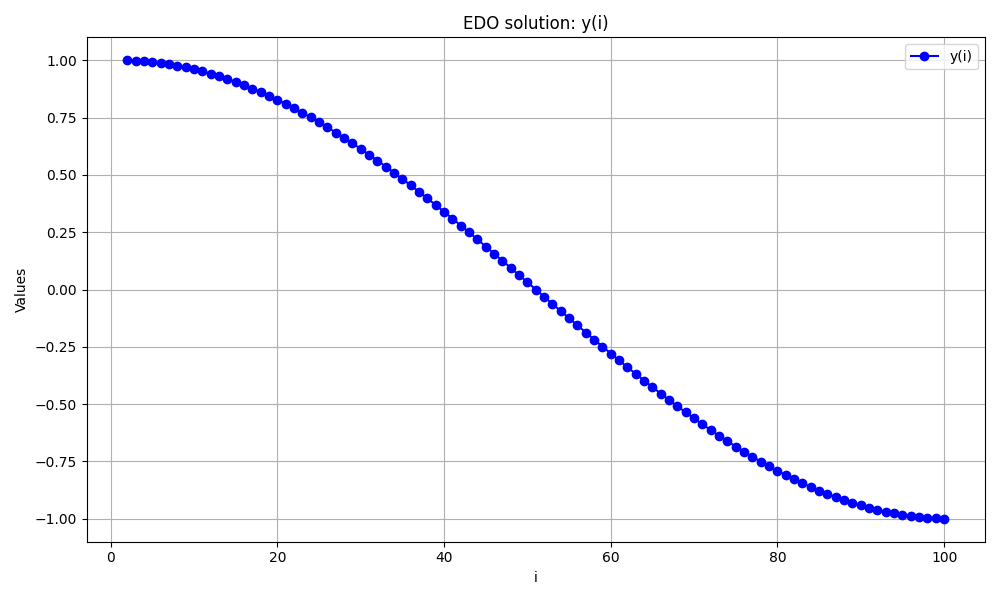
\includegraphics[width=0.8\textwidth]{../images/results-ex-3-2.png}
            \caption{Gr\'aficos de $y(x)$ e $y'(x)$ com h = 0.01}
        \end{figure}
        \begin{figure}[H]
            \centering
            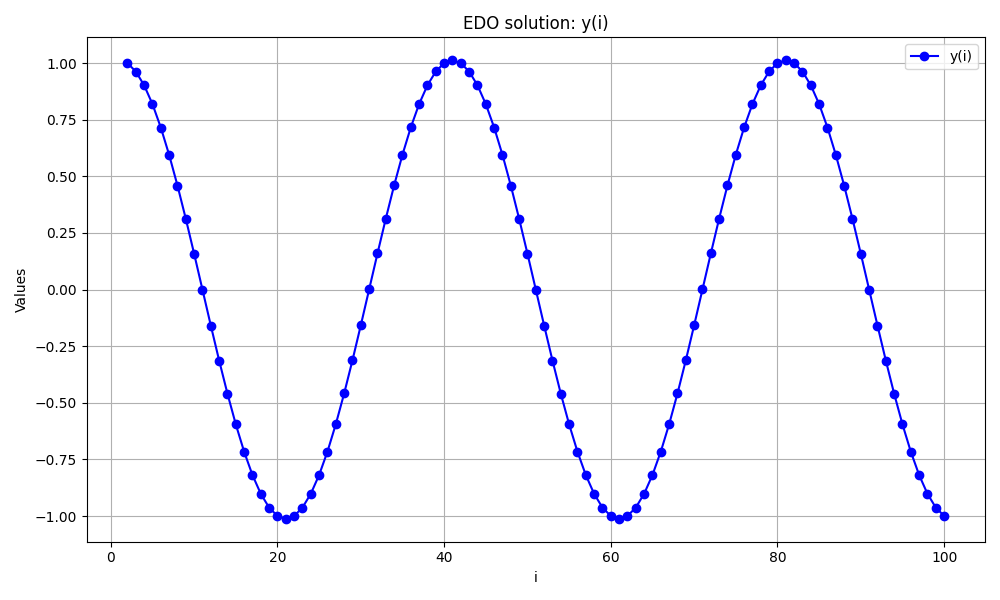
\includegraphics[width=0.8\textwidth]{../images/results-ex-3-4.png}
            \caption{Gr\'aficos de $y(x)$ e $y'(x)$ com h = 0.05}
        \end{figure}
        \begin{figure}[H]
            \centering
            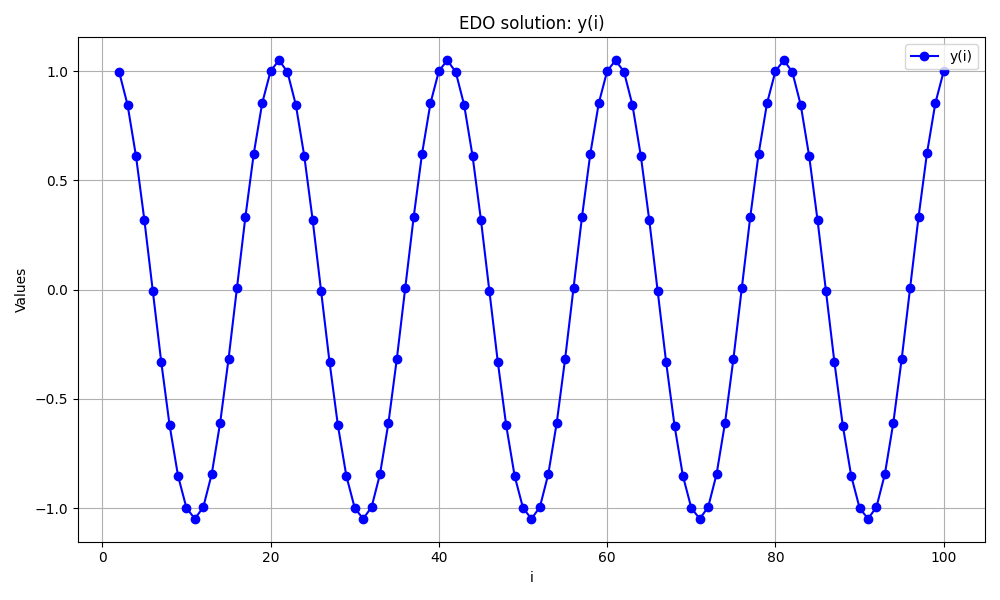
\includegraphics[width=0.8\textwidth]{../images/results-ex-3-1.png}
            \caption{Gr\'aficos de $y(x)$ e $y'(x)$ com h = 0.1}
        \end{figure}
        \begin{figure}[H]
            \centering
            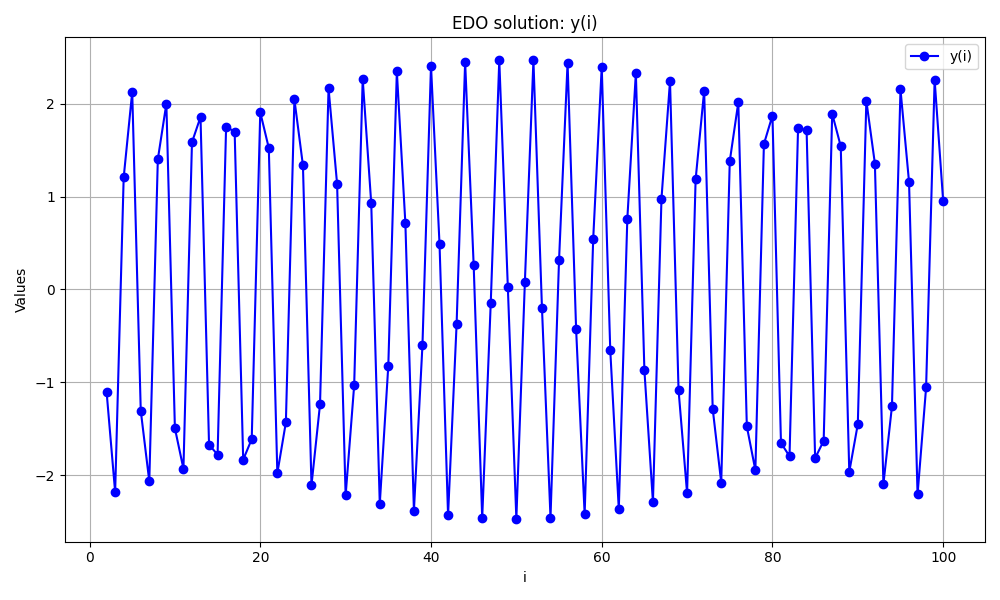
\includegraphics[width=0.8\textwidth]{../images/results-ex-3-3.png}
            \caption{Gr\'aficos de $y(x)$ e $y'(x)$ com h = 0.5}
        \end{figure}
        

        Nota-se que para os valores de h = 0.1, h = 0.01 e h = 0.05, o resultado obtido s\~ao fun\c{c}\~oes cossenoidais que oscilam de -1 a 1 o que corresponde ao comportamento esperado para a solu\c{c}\~ao da equa\c{c}\~ao diferencial. Para o valor de h = 0.5, o resultado obtido n\~ao \'e satisfat\'orio, pois a fun\c{c}\~ao n\~ao \'e cossenoidal, o que indica que o valor de h = 0.5 \'e muito grande para o algoritmo de Numerov.
        
\end{document}